
\section{Live Experiment Setup}
\label{sec:live}

We would like to perform a live demonstration of \CRATE where we would allow
WWW2016 participants to write a document together. A common goal would be
assignated to them, and possibly some sub-task would be randomly picked.

%% maybe a role playing game

%% write an introduction; write a chapter about a character; write about a city
%% make the link between two chapters; write about the end; write a plot twist
%% 
\begin{figure*}
  \centering
  \subfloat[Figure A][\label{fig:liveA} Setup of the live
  experiment. People start joining through a mediator server connected to our
  replica. It incrementally builds an editing session with browsers
  (cf. figure~\ref{fig:liveB}).]{
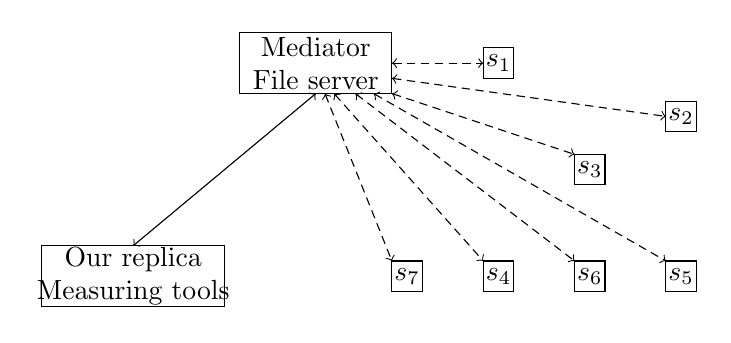
\begin{tikzpicture}[scale=1.1]
  
  \newcommand\X{30pt};
  \newcommand\Y{35pt};

  \draw[fill=white](0*\X, 0*\Y) node[align=center]{Mediator\\File server} +(-25pt,-10pt) rectangle +(25pt,10pt);
  \draw[fill=white](-2*\X, -2*\Y) node[align=center]{Our replica\\Measuring tools} +(-30pt,-10pt) rectangle +(30pt,10pt);

  \draw[fill=white](2*\X, -0*\Y)node{$s_1$} +(-5pt,-5pt) rectangle +(5pt,5pt);
  \draw[fill=white](4*\X, -0.5*\Y)node{$s_2$}  +(-5pt,-5pt) rectangle +(5pt,5pt);
  \draw[fill=white](3*\X, -1*\Y)node{$s_3$}  +(-5pt,-5pt) rectangle +(5pt,5pt);
  \draw[fill=white](2*\X, -2*\Y)node{$s_4$}  +(-5pt,-5pt) rectangle +(5pt,5pt);
  \draw[fill=white](4*\X, -2*\Y)node{$s_5$}  +(-5pt,-5pt) rectangle +(5pt,5pt);
  \draw[fill=white](3*\X, -2*\Y)node{$s_6$}  +(-5pt,-5pt) rectangle +(5pt,5pt);
  \draw[fill=white](1*\X, -2*\Y)node{$s_7$}  +(-5pt,-5pt) rectangle +(5pt,5pt);


  \draw[<->](0*\X, -10+0*\Y) -- (-2*\X, -2*\Y+10);
  \draw[<->, densely dashed] (0*\X+25,0*\Y) -- (2*\X-5, 0*\Y);
  
  \draw[<->, densely dashed] (0*\X+25,0*\Y-5) -- (4*\X-5, -0.5*\Y);
  \draw[<->, densely dashed] (0*\X+25,0*\Y-10) -- (3*\X-5, -1*\Y+5);
  \draw[<->, densely dashed] (0*\X+19,0*\Y-10) -- (4*\X-5, -2*\Y+5);
  \draw[<->, densely dashed] (0*\X+13,0*\Y-10) -- (3*\X-5, -2*\Y+5);
  \draw[<->, densely dashed] (0*\X+6,0*\Y-10) -- (2*\X-5, -2*\Y+5);
  \draw[<->, densely dashed] (0*\X+3,0*\Y-10) -- (1*\X-5, -2*\Y+5);

\end{tikzpicture}}
  \hspace{10pt}
  \subfloat[Figure B][\label{fig:liveB} Once connected, the editing session is
  autonomous. The number of connections reflects the network size. Neigbhorhoods
  are randomly filled and change over time.]{\input{input/livefigureB.tex}}
  \caption{\label{fig:live} Live demo setup.}
\end{figure*}

Figure~\ref{fig:live} depicts the demonstration setup. Figure~\ref{fig:liveA}
shows the joining process where people would open a link in their web browser
which would give them access to the editing session kept alive by \emph{Our
  replica}. Once a participant joins the editing session, it becomes part of a
network of browsers the goal of which is to create a document. Our replica,
still connected to the editing session would save the replica regularly and make
measurements about:
\begin{asparadesc}
\item [\textbf{the replicated structure size:}] depending on how the document is
  edited, the underlying sequence structure can grow heavily or remain balanced.
  \TODO{While papers often assume right-to-left editing}, human behavior is less
  predictable. Yet, we suppose that participants structure the document by
  themself and because of the given context. Such editing behavior would lead to
  a balanced data structure remaining efficient over time. 
\item [\textbf{the network:}] the traffic generated by the editing session, its
  number of participants, the average neighborhood tables size, the message rate
  over time.
\end{asparadesc}





About the web application itself, we would like to collect anonymous opinions
about:
\begin{asparadesc}
\item [\textbf{Functionality:}] were there enough functionnalities to complete
  your task?
\item [\textbf{Reliability:}] were there any trouble with the editor or the
  network?
\item [\textbf{Efficiency:}] did you feel that operations were not responding on
  time?
\item [\textbf{Communication:}] were you aware of other participants' changes?
\end{asparadesc}


%% We also would like to collect opinions on software aspects through an
%% anonymous survey. (\TODO{cf paper www2012}).

%% 1 strongly disagree -> 4 neither agree nor disagree -> 7 strongly agree

%% Functionality (suitability)
%% %% Overall, the editor supported me completing the task in a collaborative way
%% Reliablity (Maturity, recoverability)
%% %% Synchronization did not hinder my work
%% %% Page reload hinder work
%% %% on error, i recover easily
%% %% how satisfied about recover speed
%% Usability (Learnability Operability Satisfaction)
%% %% easy to learn
%% %% easy to use
%% %% actions of other did not hinder my work
%% %% overall enjoyable
%% Efficiency (Efficiency compliance)
%% %% Reponsiveness of local
%% %% Responsiveness on remote
%% %% synchronization appealing
%% Communication (Information Gathering)
%% %% presence of other participant
%% %% recognize changes on document
%% %% action of other participant
%% %% appealing editor highlighting actions
%% Coordination (Shared Access)
%% %% easily start editing at any time
%% %% edit as long as desired
%% %% editor preserved the changes i made
%% %% easily start any tool any time
%% %% '' ''  use any tool as long as desired
%% %% appealing collbarative editing

%% \TODO{What do we do with data afterwards.}

%%% Local Variables:
%%% mode: latex
%%% TeX-master: "../paper"
%%% End:
